\documentclass[graybox,vecphys]{svmult}

\usepackage{type1cm}        % activate if the above 3 fonts are
                            % not available on your system
%
\usepackage{makeidx}         % allows index generation
\usepackage{graphicx}        % standard LaTeX graphics tool
                             % when including figure files
\graphicspath{{./figures/}}
\usepackage{multicol}        % used for the two-column index
\usepackage[bottom]{footmisc}% places footnotes at page bottom
\usepackage[makeroom]{cancel}

%%% Custom commands
\newcommand{\bm}[1]{\boldsymbol{#1}}
\newcommand{\rotmat}[2]{{{ }^{#1}\boldsymbol{R}}_{#2}}
\newcommand{\ks}[1]{{(\mathrm{CS})_{#1}}}
\newcommand{\ortvek}[4]{{ }_{(#1)}{\boldsymbol{#2}}^{#3}_{#4} }
% Commands for symbol of the residual (full and reduced)
\newcommand{\Res}[0]{\vec{\delta}}
\newcommand{\ResR}[0]{\vec{\psi}}

%%% custom packages
\usepackage[T1]{fontenc}
\usepackage[utf8]{inputenc}
\usepackage{amsmath,amsfonts}
\usepackage{paralist} % for compactitem
\usepackage{url}
\usepackage{newtxtext}       % 
\usepackage[varvw]{newtxmath}       % selects Times Roman as basic font
\usepackage{subfig}
\makeindex 

\begin{document}

    \title*{Geometric Model for Serial-Chain Robot Inverse Kinematics in the Case of Two Translational DoF with Spatial Rotation and Task Redundancy}
\author{Moritz Schappler \and Tobias Blum \and Tim-David Job}
\institute{%
 All authors are with the Leibniz University Hannover, Institute for Mechatronic Systems. \email{moritz.schappler@imes.uni-hannover.de}}

%%% Provide shorter versions of title or author list if neceesary:
\titlerunning{Inverse Kinematics for Two Translational DoF with Spatial Rotation}
\authorrunning{M. Schappler et al.}

\maketitle
\vspace{-2.5cm} % space above is reserved for author affiliations. Take the space since the one affiliation is on the footer
\abstract{% 10-15 lines long
Geometric formulations for the inverse kinematics problem (IKP) in robotics are often set up in the full Cartesian space of three translational and three rotational coordinates (3T3R).
When transferring this to tasks with spatial rotation %and reduced constraints on the degrees of freedom (DoF) 
like 3T2R, 2T3R or 2T2R, the result is usually not defined in a minimal set of independent coordinates.  %when deriving their kinematics from the 3T3R formulation.
% If the kinematic model shall be formulated using a minimal set of coordinates, the excluded operational space coordinates should ideally not appear any more in the expressions.
Removing the excluded operational space coordinates completely from the expressions is interesting from a theoretical point of view and simplifies further calculations.
This can be achieved by formulating a 2R residual using the $Z$-$Y$-$X$ Tait-Bryan angles and a 2T residual derived by the projection of the pointing direction on a plane.
In this paper, the minimal-coordinate IKP is derived for 2T2R and 2T3R tasks on position level with application to a gradient-projection scheme. % and validated with a simulative example.
} 

%%% Please provide a reasonable number of keywords:
\keywords{Serial-link robot, Inverse kinematics, Task redundancy, Geometric model, Nullspace projection, Nullspace, 2T2R, 2T3R}

\section{Introduction and State of the Art}
\label{sec:introduction}

%Since research has been conducted on robotic applications, the modeling of robot structures and, in particular, inverse kinematics has been addressed \cite{GoldenbergBenFen1985}. 
%In addition to standard methods of inverse kinematics for robots with full spatial degrees of freedom (DoF) at joint and task level, extensive research has also been done on redundant robotic kinematics \cite{Yoshikawa1984}, which have more DoF in joint space than in task space. 
%The redundant DoF are not needed to perform the primary kinematic task and can be used to optimize additional criteria as a secondary task. 

%Robotic kinematics where the joint DoF exceed the physical DoF of the task space are called \emph{intrinsically} redundant. 
%If the robotic kinematics has the same DoF in the joint space and in the task space, but not all physical DoF in the operational space are needed for the task, this is called functional redundancy.

% TODO: Text oben ist zu lang. Erstelle stark verkürzten einleitenden Absatz
The inverse kinematics of robot manipulators in tasks with reduced degrees of freedom (DoF) has been investigated in the context of functional or \emph{task redundancy}, where operational and joint space have more DoF than the task space \cite{SciaviccoSic2012}.
Some tasks with axis-symmetric tools like welding \cite{Baron2000,HuoBar2008} or drilling \cite{ZanchettinRocRobJoh2011,ZhuQuCaoYan2013} require three translational and two rotational DoF (3T2R), where six-axis robots are redundant.
% Functional redundancy has already been identified and exploited by using a six-DoF robot structure. 
% This is especially the case for applications where a tool can rotate freely around it's axis of symmetry without affecting the machining process. 
%If such a task with five DoF (three translational and two rotational, 3T2R) is executed with a robot structure with six DoF, one redundant DoF remains. % \cite{Baron2000,HuoBar2008,ZanchettinRocRobJoh2011,ZhuQuCaoYan2013}. 

In some applications, the process is 
%not only independent of a rotation around a machining axis, but 
also independent of the feed in the tool axis' direction. 
This results in a task with five DoF with full orientation (2T3R) or four DoF with rotational symmetry (2T2R), which can lead to one or two redundant DoF. 
% Some applications in which the feed along an axis is free or at least limited are 
In waterjet cutting the jet can have an effective cutting range of several centimeters \cite{BahlsFroHelDeu2017}. 
Laser appliances like laser cutting \cite{DolguiPas2009} or remote laser welding \cite{ErdoesKarKem2015} can have a variable distance with a focus area or an adjustable focus point.
Other examples are drilling with a dedicated feed axis of the drilling tool \cite{KoblerKotLexMaj2014}, spraying with a range of distance \cite{FromGra2010} or the usage of a camera with a specific depth of field. 
It should be noted that in most of these 2T applications, the feed can not be disregarded as for the 2R case, but merely has to be limited to an acceptable range.
A related case are 2T constraints that occur in the remote center of motion (RCM) problem \cite{SadeghianZokJaz2019, SandovalPoiVie2017}.

The solution of the inverse kinematic problem (IKP) with functional redundancy can be obtained with the well-established nullspace-projection method \cite{SciaviccoSic2012}. 
% In order to extend this approach, which is based on the Inversion of the Jacobian, to the resolution of functional redundancies, the Jacobian must be adapted accordingly.
A requirement to use the method is the proper construction of the IK residual and the IK Jacobian.
One way is to add a virtual joint into the kinematic structure and to augment the manipulator Jacobian by one column \cite{Baron2000}. 
By adding a virtual prismatic joint the 3T2R task from \cite{Baron2000} can be transferred to a 2T2R task like in \cite{ErdoesKarKem2015} or for the RCM problem in combination with an RCM-constrained Jacobian in \cite{SadeghianZokJaz2019}.
% and even application to the RCM problem \cite{SadeghianZokJaz2019} is possible. 
The augmentation approach has the drawback that it has a higher computational cost and can lead to an ill-conditioned Jacobian \cite{HuoBar2008}.
The need of a minimal-coordinate approach is emphasized for the RCM problem in \cite{SandovalPoiVie2017}.
Another option to adapt the Jacobian is to reduce it instead of augmenting it by removing a row of the ``task frame Jacobian'' \cite{Zlajpah2017}. 
%Cartesian Jacobian \cite{ShahabiGhaBes2019} or the ``task frame Jacobian'' \cite{Zlajpah2017}. 
Reducing the Jacobian suffers from calculating the full residualand Jacobian first and removing the redundant row subsequently. 

Further solutions for the functional redundancy are based on the orthogonal decomposition of the twist \cite{HuoBar2005} or constructing a cone or pyramid with a range of tolerances for tilt angles and positions on the tool axis \cite{FromGra2010}.
Another approach uses a functional relationship between task DoF and redundant DoF for an optimized performance index via Monte-Carlo simulation \cite{ZanchettinRocRobJoh2011}.
Cascaded optimization utilizes an inner loop that solves the standard IK problem and an outer loop optimizing the performance index \cite{ZhuQuCaoYan2013}. % \cite{GuoDonKe2015}, 
The disadvantages of identifying a functional relationship \cite{ZanchettinRocRobJoh2011} is that a functional space has to be pre-defined. 
Cascaded optimization has high computational cost and does not allow using nullspace-projection method.
In \cite{MoeAntTee2016} a scalar potential is used as a constraint for a similar task, ``field of view''. 
This leads to issues with the differentiability and the convergence of the IK may suffer.
% The drawback of some of the other approaches is their high mathematical level of abstraction.

% Besides serial-chain robotic systems with full spatial motion capability, 
Parallel mechanisms with 2T2R and 2T3R reduced DoF have also been investigated, even though the case of 3T2R is more prominent. % \cite{HuangLi2003}. % \cite{Gallardo-AlvaradoArrRoj2009}. 
% Absatz zu lang:
% \cite{KumarPicBay2014} utilizes rules for joint alignments and analysis with screw theory for the synthesis of 2T3R parallel mechanisms for a medical needle holder. 
% Another possibility for the synthesis of 2T2R parallel mechanisms is based on an equivalent chain method and screw theory for oscillating screens applications \cite{YeFanGuoQu2014}. 
% \cite{ZhuHuaZha2009} uses screw theory and Grassmann geometry for synthesis of parallel robots for 2T3R tasks and singularity analysis for the application on simulation of a spinal cord in bionics. 
% The synthesis of parallel robots includes synthesis of serial leg chains and the kinematic model using screw theory. 
% This approach for modeling two translational DoF is not applicable in the IK problem for serial robots and task redundancy. 
Exemplary applications are 2T3R medical needle holders \cite{KumarPicBay2014}, 2T2R oscillating screens  \cite{YeFanGuoQu2014} or simulation of a 2T3R spinal cord in bionics \cite{ZhuHuaZha2009}.
Modeling approaches like screw theory  and Grassmann geometry are not directly applicable to the IKP in the scope of this paper.

Despite their occasional occurences in literature, the kinematics of tasks with 2T3R and 2T2R DoF are not systematically investigated for functional redundancy yet and methods for a general modeling of these tasks are sparse. 
Further, the problem is mostly formulated on velocity level which requires attention when formulating the nonlinear residual.
In this paper a general minimal-coordinate geometric approach for the position-level IKP for 2T3R and 2T2R tasks is presented. 
% The method is based on projecting the tool axis of the actual and desired end effector frame in a plane in Cartesian space, therefore the neglected DoF does not affect the residual. 
% Mathematically this is done by determining the intersection point between the projection line of this axis and the plane in Cartesian space. 
% After applying the projection on the desired frame as well as on the current frame, both of the projected points have one same entry depending on the chosen plain. 
% For the calculation of the residual by subtracting the two projected points the entries that are identical by definition and hence one translational DoF can be eliminated.
%
%
The contributions of this paper are:
\begin{compactitem}
\item a general kinematic modeling approach for inverse the kinematic problem of 2T3R and 2T2R tasks,
\item an application to the inverse kinematics with functional redundancy and redundant coordinate limitations for serial robots 
\item and an exemplary simulation.
\end{compactitem} 

% Layout: This should still be on page 2!
The outline of this paper is as follows. In Sect.\,\ref{sec:model} the proposed kinematic modeling approach for a serial chain is shown. 
The application to inverse kinematics and the resolution of functional redundancy is given in Sect.\,\ref{sec:inverse}. 
Section\,\ref{sec:simulation} demonstrates the results of the exemplary simulation and Sect.\,\ref{sec:conclusion} concludes the paper.

\section{Inverse Kinematic Model for Serial Chains}
\label{sec:model}

\begin{figure}[tb]
\centering
\input{figures/kinematic_principle.pdf_tex}
\caption{Geometric approach for the IK position (\textbf{a}) and orientation residual (\textbf{b})}
\label{fig:geometry_sketch}
\end{figure}

For robots in 2T2R and 2T3R tasks one translational DoF needs to be removed from the kinematic equations to obtain an expression of minimal dimension. 
% Analogously to the 3T2R approach \cite{SchapplerTapOrt2019a}, the $z$ axis of the end effector is defined as the tool axis in the 2T3R approach. 
This DoF is defined to be the displacement along the end effector's $z$ axis.
% For robots in 2T2R and 2T3R tasks the displacement along the end effector's $z$ axis is defined to be the redundant coordinate.
%
% Since the $z$ axis of the end effector thus always points to the target point, translation along the $z$ axis is selected as a redundant Cartesian DoF. 
The established formulation for the translational part of the inverse kinematics (IK) residual that relates the robot's joint coordinates $\vec{q}$ and operational space coordinates $\vec{x}$ is
% Thus the translational part of the inverse kinematics (IK) residual cannot be described by the established approach
\begin{equation}
\label{eq:Phi_t_3T3R}
{\Res_\mathrm{t}(\vec{q},\vec{x})} 
= 
\ortvek{0}{r}{}{DE}
=
-{_{(0)}\vec{r}_D} + {_{(0)}\vec{r}_E}(\vec{q}) = -\vec{x}_{\mathrm{t}} + {_{(0)}\vec{r}_E}(\vec{q}) ~\in {\mathbb{R}}^{3}
\end{equation}
with $\vec{x}^\transp
=
\begin{bmatrix}
\vec{x}_{\mathrm{t}}^\transp & 
\vec{x}_{\mathrm{r}}^\transp
\end{bmatrix}
= 
\begin{bmatrix}
r_{0D,x} & 
r_{0D,y} & 
r_{0D,z} & 
\varphi_x &
\varphi_y &
\varphi_z
\end{bmatrix}
\in {\mathbb{R}}^{6}$ and $\vec{x}_{\mathrm{r}}$ as Cardan angles.
% as the full spatial operational space coordinates, since it would correspond to an exact position adjustment. 
Coordinate systems are defined for the robot base $\ks{0}$, the actual end effector pose $\ks{E}$ and the desired pose $\ks{D}$, expressed with $\vec{x}$.
The residual (\ref{eq:Phi_t_3T3R}) is not feasible for the 2T case since it would correspond to an exact position adjustment.
To obtain translational redundancy, new coordinates must be chosen that allow an elimination of the redundant DoF in the residual.
The goal is to choose the coordinates $\vec{x}_t$ and $\vec{x}_r$ so that they can be reduced via selection matrices to 
$
\vec{y}_{\mathrm{t}}
=
\vec{P}_{y,\mathrm{t}}\,\vec{x}_{\mathrm{t}}$
for the 2T case and
%\quad \mathrm{and} \quad
$
\vec{y}_{\mathrm{r}}
=
\vec{P}_{y,\mathrm{r}}\,\vec{x}_{\mathrm{r}}
$
for the 2R case.
%\begin{equation}
%\vec{y}
%=
%\begin{bmatrix}
%\vec{y}_{\mathrm{t}}^\transp & 
%\vec{y}_{\mathrm{r}}^\transp
%\end{bmatrix}^\transp = \begin{bmatrix}
%(\vec{P}_{y,\mathrm{t}}\,\vec{x}_{\mathrm{t}})^\transp &
%(\vec{P}_{y,\mathrm{r}}\,\vec{x}_{\mathrm{r}})^\transp
%\end{bmatrix}^\transp = \vec{P}_{y}\,\vec{x}
%\end{equation}  
%by removing entries via permutation/selection matrices $\vec{P}_{y,\mathrm{t}}$ and $\vec{P}_{x,\mathrm{t}}$. 
By stacking the translational and rotational coordinates the combinations 2T2R and 2T3R (and also 3T2R or 3T3R) can be created. 
%For a 2T2R task the the reduced coordinates $\vec{y}^\transp
%=
%\begin{bmatrix}
%\vec{y}_{\mathrm{t}}^\transp & 
%\vec{y}_{\mathrm{r}}^\transp
%\end{bmatrix}$ are used.

In this approach the translational task \emph{minimal} coordinates are chosen as 
\begin{equation}
\label{eq:minimalkoordinaten_2T}
\vec{y}_{\mathrm{t}}
=
\begin{bmatrix}
r_{0D',x}  & r_{0D',y}
\end{bmatrix}^\transp
=
%\underbrace{\begin{bmatrix}
%1 & 0 & 0  \\ 
%0 & 1 & 0
%\end{bmatrix}}_{=\vec{P}_{y,\mathrm{t}}}
\vec{P}_{y,\mathrm{t}}
\begin{bmatrix}
r_{0D',x} & 
r_{0D',y} & 
{\lambda_{D'}}
\end{bmatrix}^\transp
\in {\mathbb{R}}^{2},
\end{equation}  
%
where the index $D'$ in $r_{0D',x}$ and $r_{0D',y}$ refers to the intersection of the $z$ axis of $\ks{D}$ with the $x$-$y$ plane of $\ks{0}$ shown in Fig.~\ref{fig:geometry_sketch},a and $\lambda_{D'} = {_{(D)}r_{DD',\mathrm{z}}}$ is the distance to this intersection point which is derived in the following. 

The point $E'$ is obtained similarly from $\ks{E}$ by setting up a line equation %${\vec{g}(\vec{q})}$ 
\begin{equation}
\label{eq:equation_system}
{\vec{g}(\vec{q})}
={_{(0)}\vec{r}_E(\vec{q})}+ {\lambda{_{(0)}\vec{e}_{\mathrm{z}}^{E}}(\vec{q})}
%=
%{_{(0)}\vec{r}_{E'}(\vec{q})}
%=
%{\bm{p}(\vec{q})}
\end{equation}
from the vector of location ${_{(0)}\vec{r}_E(\vec{q})}$
% which corresponds to the current position of $\ks{E}$ 
in the direction of the $z$ axis $\vec{e}_{\mathrm{z}}^{E}(\vec{q})$ % from the orientation 
of $\ks{E}$.
% To calculate the intersection point, ${\vec{g}(\vec{q})}$ is equate with the $xy$ plane ${\bm{p}(\vec{q})}$ by a system of equations
%
%\begin{equation}
%\label{eq:GLS_Schnitt_XY}
%{\bm{\mathit{g}}(\vec{q})} 
%=
%\begin{bmatrix}
%r_{0E',x}(\vec{q}) \\
%r_{0E',y}(\vec{q}) \\
%0 \\
%\end{bmatrix}
%=
%\begin{bmatrix}
%r_{0E,x}(\vec{q}) \\
%r_{0E,y}(\vec{q}) \\
%r_{0E,\mathrm{z}}(\vec{q}) \\
%\end{bmatrix}
%+ \lambda
%\begin{bmatrix}
%{e_\mathrm{z,x}^E}(\vec{q}) \\
%{e_\mathrm{z,y}^E}(\vec{q}) \\
%{e_\mathrm{z,z}^E}(\vec{q}) \\
%\end{bmatrix}
%\end{equation}
The intersection
${_{(0)}\vec{r}_{E'}}%=\begin{bmatrix}
%r_{0E',x} & 
%r_{0E',y} & 
%r_{0E',z} 
%\end{bmatrix}
$
of the line in (\ref{eq:equation_system}) with the $x$-$y$ plane of $\ks{0}$ is obtained by
% To solve the equation system, $\lambda$ is obtained by the last row of (\ref{eq:equation_system}) through rearranging it to
\begin{equation}
\label{eq:lambda_Edash}
{\lambda(\vec{q})} 
= 
{\lambda_{E'}(\vec{q})} 
= 
\left(0 - r_{0E,\mathrm{z}}(\vec{q})\right)/{e_\mathrm{z,z}^E}(\vec{q}) 
= 
-r_{0E,z}(\vec{q}) / e_{z,z}^E(\vec{q}).
\end{equation}

% Layout: The page should end with this equation above

Inserting ${\lambda_{E'}}$ in $\vec{g}(\vec{q})$ gives ${_{(0)}\vec{r}_{E'}}$, which is also sketched in Fig.~\ref{fig:geometry_sketch},a.
%\begin{equation}
%\label{eq:r_0E'}
%{_{(0)}\vec{r}_{E'}}(\vec{q}) = 
%{_{(0)}\vec{r}_{E}(\vec{q})}+ %{\lambda_{E'}(\vec{q}){_{(0)}\vec{e}_{\mathrm{z%}}^E}(\vec{q})}
%\end{equation}
% This point corresponding to $E'$ from Fig.~\ref{fig:geometry_sketch},a and 
The variable ${\lambda_{E'}}$ can be understood as the distance from $\ks{E}$ to $E'$. %, form the first part of the translational residual. 
% The point of intersection $D'$
% %, respectively ${_{(0)}\vec{r}_{D'}}$, and ${\lambda_{D'}}$ 
% can be calculated analogously. %, only depending on reduced coordinates $\vec{y}$.

With the new coordinates corresponding to (\ref{eq:minimalkoordinaten_2T}), the translational residual 
\begin{equation}
\label{eq:Phit}
\Res_\mathrm{t}(\vec{q},\vec{x})
=
\begin{bmatrix}
-r_{0D',x}(\vec{x}) + r_{0E',x}(\vec{q}) \\
-r_{0D',y}(\vec{x}) +r_{0E',y}(\vec{q}) \\
- {\lambda_{D'}(\vec{x})} + {\lambda_{E'}(\vec{q})} \\
\end{bmatrix}
\end{equation}
is now defined. % as the distance between them. 
The reduced residual for 2T tasks can be obtained through
\begin{equation}
\label{eq:Psit_2T}
\ResR_\mathrm{t}(\vec{q},\vec{y}) = %\overbrace{\begin{bmatrix}
%    1 & 0 & 0  \\ 
%    0 & 1 & 0
%    \end{bmatrix}}^{=\vec{P}_{\ResR,\mathrm{t}}}
\begin{bmatrix}
    1 & 0 & 0  \\ 
    0 & 1 & 0
    \end{bmatrix}
 \Res_\mathrm{t}(\vec{q},\vec{x})
 =\vec{P}_{\ResR,\mathrm{t}} \Res_\mathrm{t}(\vec{q},\vec{x})
 ~\in {\mathbb{R}^2}.
\end{equation} 
%by multiplying a permutation matrix $\vec{P}_{\ResR,\mathrm{t}}$. 
The peculiarity of the kinematic model lies in the sole dependency on the reduced coordinates $\vec{y}$.
For the solution of the IKP shown in Sect.\,\ref{sec:inverse} the gradient of the residual w.r.t. $\vec{q}$ is needed.
It follows by partial derivation (and by ignoring the third row) to
\begin{align}
{\frac{\partial}{\partial\vec{q}}\ResR_\mathrm{t}}(\vec{q},\vec{x}) &= \vec{P}_{\ResR,\mathrm{t}} {\Big(\frac{\partial}{\partial\vec{q}}{_{(0)}\vec{r}_{0E'}(\vec{q})}\Big)} \nonumber\\ &= \vec{P}_{\ResR,\mathrm{t}}
{\Big(\frac{\partial}{\partial\vec{q}}{_{(0)}\vec{r}_{0E}(\vec{q})}} + 
{\frac{\partial}{\partial\vec{q}}\big({\lambda_{E'}(\vec{q})}{_{(0)}\vec{e}_{\mathrm{z}}^E}(\vec{q})\big)\Big)} \label{eq:Phi_grad_2T2R_1}\\ &= \vec{P}_{\ResR,\mathrm{t}}
{\Big(\frac{\partial}{\partial\vec{q}}{_{(0)}\vec{r}_{0E}(\vec{q})}} + 
{\frac{\partial{\lambda_{E'}(\vec{q})}}{\partial\vec{q}}}{_{(0)}\vec{e}_{\mathrm{z}}^E}(\vec{q}) +
{{\lambda_{E'}(\vec{q})}\frac{\partial{_{(0)}\vec{e}_{\mathrm{z}}^E}(\vec{q})}{\partial\vec{q}}\Big)}. \label{eq:Phi_grad_2T2R_2}
\end{align}
%
Since ${\lambda_{E'}(\vec{q})}$ from (\ref{eq:lambda_Edash}) is the quotient of  ${f_\mathrm{1}(\vec{q})} = {-{r_{0E,\mathrm{z}}(\vec{q})}}$ and ${f_\mathrm{2}(\vec{q})} = {e_\mathrm{z,z}^E(\vec{q})}$, dependent on $\vec{q}$, it's partial derivative is calculated by the quotient rule for differential calculus.
% \begin{align}
% \frac{\partial{\lambda_{E'}(\vec{q})}}{\partial\vec{q}} = \frac{\partial}{\partial\vec{q}}\frac{{f_\mathrm{1}(\vec{q})}}{{f_\mathrm{2}}(\vec{q})} = 
%\frac{f_\mathrm{2}(\vec{q})\frac{\partial{f_\mathrm{1}}(\vec{q})}{\partial\vec{q}} - f_\mathrm{1}(\vec{q})\frac{\partial{f_\mathrm{2}}(\vec{q})}{\partial\vec{q}}}{{f_\mathrm{2}^2}(\vec{q})} \label{eq:lambda_Edash_dq}\\
% \mathrm{with} \quad {f_\mathrm{1}(\vec{q})} = {-{r_{0E,\mathrm{z}}(\vec{q})}}\nonumber
% \quad \mathrm{and} \quad
% {f_\mathrm{2}(\vec{q})} = {e_\mathrm{z,z}^E(\vec{q})}. \nonumber
% \end{align}
%with the help of the quotient rule. 
The term ${\partial{\vec{e}_{\mathrm{z}}^\mathrm{E}}(\vec{q})}/{\partial\vec{q}}$ in $f_\mathrm{2}$ can be obtained either by symbolic derivation using computer algebra systems or by a relation with the rotational part of the geometric Jacobian, which can be derived with the methods from \cite{SchapplerTapOrt2019a}. %the relation between rotation matrices and angular velocities together with the rotational part of the geometric Jacobian and rules for differentiation of stacked rotation matrices discussed in \cite{SchapplerTapOrt2019a}.

The rotational residual is calculated using the $Z$-$Y$-$X$ Tait-Bryan angles
\begin{equation}
\Res_{\mathrm{r}}(\vec{q},\vec{x})
=
\vec{\alpha}\left(\rotmat{D}{E}(\vec{q},\vec{x}_{\mathrm{r}})\right)
=
\vec{\alpha}\left(\rotmat{0}{D}^\transp (\vec{x}_{\mathrm{r}})\rotmat{0}{E}(\vec{q})\right)
=[\alpha_z,\alpha_y,\alpha_x]^\transp
~\in {\mathbb{R}^3}.
\end{equation}
The series of elementary rotations is depicted in Fig.~\ref{fig:geometry_sketch},b.
By explicitely adding two intermediate frames $\ks{A1}$ and $\ks{A2}$ that share the same $z$ axis with the desired frame $\ks{D}$, the purpose of this angle convention becomes apparent. 
Since the rotation around this axis is the redundant DoF these frames with elementary rotations $\varphi_z$ and $\alpha_z$ can be omitted for the reduced residual, which is sketched by the dashed line to $\ks{A2}$. %The rotational residual 
%\begin{equation}
%\Res_{\mathrm{r}}(\vec{q},\vec{x})
%=
%\vec{\alpha}\left(\rotmat{A2}{E}(\vec{q},\vec{y}_{\mathrm{r}},\alpha_z,\varphi_z)\right)
%=
%\vec{\alpha}\left(\rotmat{0}{A1}^\transp (\vec{y}_{\mathrm{r}},\alpha_z,\varphi_z)\rotmat{0}{E}(\vec{q})\right)
%~\in {\mathbb{R}^3}
%\end{equation}
%can be obtained by a set of Z-Y-X Euler angles $\vec{\alpha}$. 
Analogously to (\ref{eq:Psit_2T}), multiplying a permutation matrix  leads to the reduced residual $\ResR_\mathrm{r}(\vec{q},\vec{y}) = \vec{P}_{\ResR,\mathrm{r}} \Res_{\mathrm{r}}(\vec{q},\vec{x})~\in {\mathbb{R}^2}$ for 2R tasks. For the derivation of the gradient and details of this approach refer to \cite{SchapplerTapOrt2019a}. 

Similiar to the coordinate definitions $\vec{y}$ and $\vec{x}$, the full residual
$
\ResR(\vec{q},\vec{y})^\transp = \begin{bmatrix}
(\vec{P}_{\ResR, \mathrm{t}}\Res_\mathrm{t}(\vec{q},\vec{x}))^\transp &
(\vec{P}_{\ResR, \mathrm{r}}\Res_\mathrm{r}(\vec{q},\vec{x}))^\transp
\end{bmatrix}
$
is obtained by stacking the translational and rotational residual in any combination depending on the task DoF (2T2R, 2T3R, ...) by chosing the according permutation matrix. 
%For a 2T2R task the residual is chosen as  $\ResR(\vec{q},\vec{y})^\transp = \begin{bmatrix}
%\ResR_t(\vec{q},\vec{y})^\transp &
%\ResR_r(\vec{q},\vec{y})^\transp
%\end{bmatrix}$.





\section{Inverse Kinematics and Task Redundancy}
\label{sec:inverse}

%\begin{compactitem}
%\item Formulierung des IKP und Newton-Raphson-Algorithmus mit Nullraum-Projektion
%\item Beispiele für Potentialfunktionen für Nullraumkriterien (Gelenkwinkel-Grenzen, 
%\item Ausblick: Kaskadierte Nullraumoptimierung: Erst Nebenbedingungen, dann eigentliche Optimierung (Noch offener Arbeitspunkt)
%\end{compactitem}
The solution of the inverse kinematics problem can be obtained through the Newton-Raphson method derived by the Taylor series of the IK residual $\ResR(\vec{q},\vec{y})$ to
\begin{equation}
\ResR(\vec{q}^{k+1},\vec{y}) =
\ResR(\vec{q}^{k},\vec{y})
+
\ResR_{\partial \vec{q}}(\vec{q}^k,\vec{y}) (\vec{q}^{k+1} - \vec{q}^k)
\overset{!}{=}
\vec{0}
\end{equation}
with the IK Jacobian matrix $\ResR_{\partial \vec{q}}(\vec{q}^k,\vec{y})$. 
With $\dagger$ for pseudo inverse, 
%With condition $\ResR(\vec{q}^{k+1},\vec{y}) = \vec{0}$ 
the increment
\begin{equation}
\Delta \vec{q}^k
=
(\vec{q}^{k+1} - \vec{q}^k)
=
- 
\left(\ResR_{\partial \vec{q}}(\vec{q},\vec{y})\right)^{\dagger}
\ResR(\vec{q}^{k},\vec{y})
\label{equ:deltaq_psi}
\end{equation}
of the joint angles can be used in an iterative algorithm to move towards the solution. 
Secondary tasks $\bm{v}{=}h_{\partial\vec{q}}$ can be optimized in the nullspace of the operational task via
\begin{align}
{\Delta}\vec{q}
=
{\Delta}\vec{q}_{\mathrm{T}} + {\Delta}\vec{q}_{\mathrm{N}}
=
-\ResR_{\partial\vec{q}}^{\dagger} \ResR +  \vec{N} \bm{v}
\quad \mathrm{with} \quad
\vec{N}=\vec{I}-\ResR_{\partial\vec{q}}^{\dagger}\ResR_{\partial\vec{q}}
\label{equ:nullspace}
\end{align}
using the gradient-projection method.
To focus on the geometric derivation of the residual, using multiple optimization criteria as shown in \cite{MoeAntTee2016} is not considered.

The distance of robot end effector to workpiece in pointing direction $d_z$ is obtained from the vector $\ortvek{D}{r}{\transp}{DE} = [d_x,d_y,d_z]$ shown in Fig.~\ref{fig:geometry_sketch},a.
The reference distance of the robot can be limited e.g. by the task specification to be within the bounds $d_{z,\mathrm{min}}$ to $d_{z,\mathrm{max}}$.
To respect these bounds the modified hyperbolic potential function
%
\begin{equation}
h_{d_z,\mathrm{hyp}}(d_z)
=
\frac{(d_{z,\mathrm{max}}-d_{z,\mathrm{min}})^2}{8}
\left(
\frac{1}{(d_{z}-d_{z,\mathrm{min}})^2}
+
\frac{1}{(d_{z}-d_{z,\mathrm{max}})^2}
\right)
\ge 1
\label{equ:h_dz_hyp}
\end{equation}
%
from \cite{ZhuQuCaoYan2013}
can be used.
%
Cubic splines serve for activation of the potential at the thresholds $d_{z,\mathrm{thr,min}}$ and $d_{z,\mathrm{thr,max}}$. 
The switch from spline to hyperbolic potential is done at $d_{z,\mathrm{sw,min}}$ and $d_{z,\mathrm{sw,max}}$ and provides a continuously differentiable potential.
This results in the piecewise defined potential
%
\begin{equation}
h_{\mathrm{dist}}(h_{d_z})
=
\begin{cases} 
h_{d_z,\mathrm{hyp}} & \mathrm{for} \quad \hphantom{d_{z,\mathrm{sw,min}}} \hphantom{\leq} d_z \leq d_{z,\mathrm{sw,min}} \\
h_{d_z,\mathrm{spline,ll}} & \mathrm{for} \quad d_{z,\mathrm{sw,min}} \leq d_z\leq d_{z,\mathrm{thr,min}} \\
0 & \mathrm{for} \quad d_{z,\mathrm{thr,min}} \leq d_z\leq d_{z,\mathrm{thr,max}} \\
h_{d_z,\mathrm{spline,ul}} & \mathrm{for} \quad d_{z,\mathrm{thr,min}} \leq d_z \leq d_{z,\mathrm{sw,max}} \\
h_{d_z,\mathrm{hyp}} & \mathrm{for} \quad d_{z,\mathrm{sw,max}} \leq d_z.
\end{cases}.
\label{equ:h_dist_pw}
\end{equation}

A symbolic derivation of the residual w.r.t. $\vec{q}$ is not feasible.
Instead, the gradient is computed with the projection of the known expression $\partial h(d_z)/\partial d_z$ as
%
\begin{equation}
h_{\partial \vec{q}}^{*} 
= 
\frac{\partial h}{\partial d_z} 
\frac{\partial d_z}{\partial \vec{q}}.
\label{eq:grad_proj_dqdz}
\end{equation}

The asterisk denotes the origin of the term from a projection approach instead of a symbolic derivation.
Using symbolic derivation leads to a different expression $h_{\partial \vec{q}}$, but after projection into the nullspace of the IK Jacobian in (\ref{equ:nullspace}), both gradients are equal, i.e. $\vec{N} h_{\partial \vec{q}}=\vec{N} h_{\partial \vec{q}}^{*} $.
The second term in (\ref{eq:grad_proj_dqdz}) comes from the last row of the rotated translational part ${_{(D)}\vec{J}_\mathrm{t}}$ of the robot's Jacobian.
A rotation from default base frame $\vec{J}_\mathrm{t}{:=}{_{(0)}\vec{J}_\mathrm{t}}$ into desired frame is performed with
\begin{equation}
{_{(D)}\vec{J}_\mathrm{t}} 
= 
\rotmat{D}{0} {_{(0)}\vec{J}_\mathrm{t}}
=
\rotmat{D}{0}
\frac{\partial}{\partial \vec{q}} \ortvek{0}{r}{}{E}
=
\frac{\partial}{\partial \vec{q}} 
\rotmat{D}{0}
(\ortvek{0}{r}{}{D} {+} \ortvek{0}{r}{}{DE})
=
\frac{\partial}{\partial \vec{q}} \ortvek{D}{r}{}{DE}.
\label{eq:jacobian_rotation}
\end{equation}

The relations hold since $\rotmat{D}{0}$ and $\ortvek{0}{r}{}{D}$ are only dependent on the desired pose $\vec{x}$ and not on the joint configuration $\vec{q}$ and are invariant to the operator $\partial/\partial \vec{q}$.
Generally spoken, the Jacobian relation is invariant to the reference frame.
Therefore $\partial d_z / \partial \vec{q}$ in (\ref{eq:grad_proj_dqdz}) can be obtained as the last row of the Jacobian ${_{(D)}\vec{J}_\mathrm{t}}$ from (\ref{eq:jacobian_rotation}).

Other performance criteria can be included like a potential from \cite{HuoBar2008} based on the squared deviation of the joint coordinate $\vec{q}$ from their mid-range $\bar{\vec{q}}$ with

\begin{equation}
h_1(\vec{q})
=
\frac{1}{2} (\vec{q}-\bar{\vec{q}})^\transp\vec{W}_1(\vec{q}-\bar{\vec{q}}),
\quad
h_{1,\partial\vec{q}}
=
\frac{\partial h_1}{\partial \vec{q}}
=
\vec{W}_1(\vec{q}-\bar{\vec{q}}) 
\quad \mathrm{and} \quad \vec{W}_1=\vec{I}.
\label{equ:h_qlim_par}
\end{equation}

Both criteria are combined to one potential $h_{\mathrm{total}}=h_{\mathrm{dist}} + h_1$.
Other criteria like singularity avoidance \cite{HuoBar2008} or hyperbolic weight of joint limit distance \cite{ZhuQuCaoYan2013} can be used as well.
If e.g. for 2T2R tasks a two-DoF task redundancy arises, a task-priority scheme \cite{MoeAntTee2016} can be used to incorporate several objectives simultaneously.

\section{Simulative Evaluation}
\label{sec:simulation}


\begin{figure}[b]
\centering
\input{figures/robots_ik_results.pdf_tex}
\caption{Robot in initial pose (\textbf{a}) and in final poses for different IK settings (\textbf{b}--\textbf{e})}
\label{fig:robots_ik_results}
\end{figure}

\begin{figure}[b]
\begin{center}
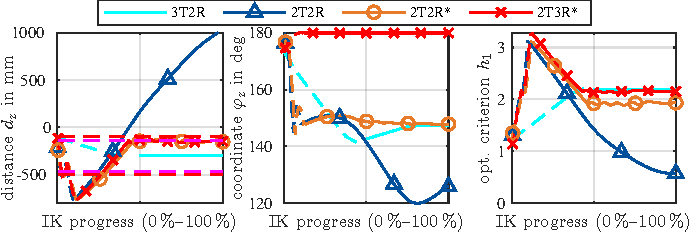
\includegraphics[]{figures/ik_results.pdf}
\caption{Target distance $d_z$ with threshold $d_{z,\mathrm{thr,min/max}}$ and limit $d_{z,\mathrm{min/max}}$ (\textbf{a}), end effector rotation $\varphi_z$ corresponding to $\ks{E}$ (\textbf{b}) and joint limit optimization criterion $h_1$ (\textbf{c}) over the convergence of the IK algorithm. Dashed lines mark $\Res \napprox \vec{0}$}
\label{fig:ik_results}
\end{center}
\end{figure}


A simulation study was performed with the proposed algorithm for an industrial robot kinematics of type KUKA KR 30-3.
The initial robot pose is shown in Fig.~\ref{fig:robots_ik_results},a together with the desired pose $\ks{D}$ and limitations for the redundant coordinate $d_z$ in the 2T tasks. \\
Different settings of the IK algorithm were used with summed optimization of the criterion $h_1$ from (\ref{equ:h_qlim_par}) and $h_\mathrm{dist}$ from (\ref{equ:h_dist_pw}).
The resulting final poses for each setting are shown in Fig.~\ref{fig:robots_ik_results},b--e.
The evolution of the redundant translational coordinate $d_z$ (in the 2T case) and the redundant rotational coordinate $\varphi_z$ regarding the $z$ axis (in the 2R case) are plotted in Fig.~\ref{fig:ik_results},a--b.
From Fig.~\ref{fig:ik_results},c the optimization criterion $h_1$ can be estimated.
The IK progress is normalized from 0 to 100\,\%.
However, the number of iterations $k$ varies from 18 (3T2R), over 232 (2T2R) and 308 (2T3R*) to 539 (2T2R*) and depends on the maximum step size and other meta parameters in the implementation of (\ref{equ:deltaq_psi}).

In the 2T2R case, without limiting the coordinate $d_z$
% with residual from (\ref{eq:Psit_2T}) and (\ref{eq:Psit_2R}) 
the functional redundancy of degree two is used only for a far reaching elongation of the arm in Fig.~\ref{fig:robots_ik_results},c.
This strongly improves $h_1$, but is infeasible regarding collisions, singularities and possible process restrictions.
This is improved by the method 2T2R* which uses $h_1+h_\mathrm{dist}$ at the cost of a degraded $h_1$, see Fig.~\ref{fig:robots_ik_results},d.
Using a fixed orientation $\varphi_z$ with 2T3R* does not allow to improve $h_1$ further since the one degree of functional redundancy is already used for $h_\mathrm{dist}$ which is at it's limit as can also be seen in Fig.~\ref{fig:robots_ik_results},e.
Finally, for comparison, the case of 3T2R in Fig.~\ref{fig:robots_ik_results},b is included with a shifted $\ks{D}$ in the middle of $d_{z,\mathrm{min}}$ and $d_{z,\mathrm{max}}$, which allows optimization of $h_1$ to a poorer result than the other methods due to the reduced range of self-motion.

\section{Conclusion}
\label{sec:conclusion}

The proposed formulation for definition of the inverse kinematics problem can be used for tasks with two translational degrees of freedom and spatial motion, especially 2T2R and 2T3R.
The method is targeted at a numeric implementation.
Extensions such as the limitation of the redundant coordinate with a projection method make it more feasible in practical applications.
The minimal dimension of the residual and the elimination of dependent operational space coordinates allow an efficient transfer to parallel robots and other applications.
% The approach can further be used for the inverse kinematics model of parallel robots
%--- either for optimization in task redundancy or for synthesis of parallel robots with structurally 2T2R and 2T3R DoF.

% A next step for the application of the approach is using it for the IK model of parallel robots either with task redundancy or with structurally 2T2R and 2T3R DoF.

\begin{acknowledgement}
The authors acknowledge the support by the Deutsche Forschungsgemeinschaft (DFG) under grant number 341489206. \textsc{Matlab} code to reproduce the results
is available at GitHub under free license at \url{github.com/SchapplM/robotics-paper_ark2022_2T2R}.
\end{acknowledgement}

\bibliographystyle{spmpsci}
\bibliography{references}

\end{document}
